\documentclass[11pt, a4paper]{article}
\usepackage[english]{babel}
\usepackage[utf8]{inputenc}
\usepackage{fancyhdr}
\usepackage{lastpage}
\usepackage{datetime}
\usepackage{indentfirst}
\usepackage{hyperref}
\usepackage{appendix}
\usepackage{amsmath}
\usepackage{amssymb}
\usepackage{amsfonts}
\usepackage{mathtools}
\usepackage{siunitx}
\usepackage{cancel}
\usepackage{tabularray}
\usepackage{multirow}
\usepackage{array}
\usepackage{hhline}
\usepackage{makecell}
\usepackage{courier}
\usepackage[font=small, skip=0pt]{caption}
\usepackage[font=scriptsize, skip=0pt]{subcaption}
\usepackage{float}
\usepackage{graphicx}
\usepackage{listings}
\usepackage{xcolor}
\usepackage{matlab-prettifier}
\usepackage[T1]{fontenc}
\usepackage{lmodern}
\usepackage{bigfoot}
\usepackage{filecontents}
\usepackage[nottoc]{tocbibind}

\graphicspath{ {./mathimages/} }

\newdateformat{Datea}{\THEDAY\ \monthname[\THEMONTH] \THEYEAR}
\newdateformat{Dateb}{\monthname[\THEMONTH] \THEYEAR}

%\allowdisplaybreaks
\DeclareMathOperator{\cosec}{cosec}
\DeclareMathOperator{\cotan}{cotan}
\DeclareMathOperator{\sech}{sech}
\DeclareMathOperator{\cosech}{cosech}
\DeclareMathOperator{\arcsec}{arcsec}
\DeclareMathOperator{\arccot}{arccot}
\DeclareMathOperator{\arccsc}{arccosec}
\DeclareMathOperator{\arccosh}{arccosh}
\DeclareMathOperator{\arcsinh}{arcsinh}
\DeclareMathOperator{\arctanh}{arctanh}
\DeclareMathOperator{\arcsech}{arcsech}
\DeclareMathOperator{\arccsch}{arccsch}
\DeclareMathOperator{\arccoth}{arccoth}
\DeclareMathOperator{\arsinh}{arsinh}
\DeclareMathOperator{\arcosh}{arcosh}
\DeclareMathOperator{\artanh}{artanh}

\DeclareMathOperator{\cis}{cis}

\pagestyle{fancy}
\fancyhf{}
\rhead{Hatam Barma}
\chead{\begin{tabular}[t]{@{}l@{}}\\Mathematics and Further Mathematics Pure Revision Summary\end{tabular}}
\lhead{\Dateb\today}
\cfoot{Page \thepage}

\renewcommand{\thesection}{\arabic{section}} 

\renewcommand{\thesubsection}{\thesection.\arabic{subsection}}

\setcounter{section}{0}

\allowdisplaybreaks

\fancypagestyle{plain}{
\fancyhf{}
\renewcommand{\headrulewidth}{0pt}}

\hypersetup{
    colorlinks,
    citecolor=black,
    filecolor=black,
    linkcolor=blue,
    urlcolor=magenta!70!black
}

\begin{document}


\begin{titlepage}
   \begin{center}
       \vspace*{2.5cm}
	\huge
       \textbf{A-Level Mathematics and Further Mathematics Pure Revision Summary} \\
	\vspace{1cm}
	\Large
       \textbf{Chapter 1: Functions and coordinate systems}
            
       \vspace{1.5cm}
	\LARGE
       \textbf{Hatam Barma} \\
	\vspace{0.75cm}
       \normalsize
       \emph{Compiled on \Datea\today} \\

       \vfill
        

	E-mail: hatam.barma@gmail.com
   \end{center}
\end{titlepage}


\tableofcontents

\clearpage
\section{Functions and coordinate systems}
\vspace{0.5cm}

\subsection{The fundamental theorem of algebra}
\label{fundtheory}
\begin{itemize}
\item A Level M AS / Year 1 \hspace{1cm} \phantom{ } Pages 59 -- 62
\item A Level M Year 2 \hspace{1cm} \phantom{ AS / } Pages 93 -- 99
\item A Level FM AS / Year 1 \hspace{1cm} Pages 141 -- 159
\end{itemize} \par
For any polynomial of degree $n$, with real $(\mathbb{R})$ coefficients, it can be factorised into $n$ linear real roots and \ or complex roots, and for any given complex root $(z)$, its conjugate $(z^{*})$ is also a root. Where $z$ is a complex number, $zz^{*}$ gives a real quadratic, and so the polynomial can be written as a product of real linear and / or irreducible quadratic factors.
\begin{itemize}
\item[Note:] $\left( z^{*} \right)^{n} = \left( z^{n} \right)^{*}$
\end{itemize}
\vspace{0.5cm}

\subsection{Radian measure}
\label{radianmeasure}
\begin{itemize}
\item A Level M Year 2 \hspace{1cm} \phantom{ AS / } Pages 128 -- 134
\item A Level M Year 2 \hspace{1cm} \phantom{ AS / } Pages 147 -- 155
\end{itemize} \par
The radian is the SI unit of measurement for angles, and is in many ways a more intuitive measure of angles. The magnitude of an angle in radians is defined as the ratio between the arc length that the angle subtends, and the radius of the circle. \newline \par

\noindent $Angle\; in\; radians = \frac{arc\; length}{radius}$ \hspace{2cm} Radians are dimensionless \newline
$Arc\; length = radius\times angle\; (in\; radians) = r\theta$ \newline
$Sector\; area = \pi r^{2}\times\frac{\theta}{2\pi}=\frac{1}{2}r^{2}\theta$ \newline \par

It is very worthwhile becoming familiar with radians, and they should feel as natural to use as degrees. In the same way you learnt standard trigonometric values for  some useful angles at GCSE, you should learn these same values with radians.

\begin{center}
\begin{tblr}{|[.75pt]|c|c||c|c|c||[.75pt]}
\hline[1.25pt]
$\theta$ in $^{\circ}$ & $\theta$ in radians & $\sin(\theta)$ & $\cos(\theta)$ & $\tan(\theta)$ \\ \hline[1pt]
$0$ & $0$ & $0$ & $1$ & $0$ \\ \hline
$30$ & $\frac{\pi}{6}$ & $\frac{1}{2}$ & $\frac{\sqrt{3}}{2}$ & $\frac{1}{\sqrt{3}}$ \\ \hline
$45$ & $\frac{\pi}{4}$ & $\frac{1}{\sqrt{2}}$ & $\frac{1}{\sqrt{2}}$ & $1$ \\ \hline
$60$ & $\frac{\pi}{3}$ & $\frac{\sqrt{3}}{2}$ & $\frac{1}{2}$ & $\sqrt{3}$ \\ \hline
$90$ & $\frac{\pi}{2}$ & $1$ & $0$ & $\mathrm{undefined}$ \\ \hline[.75pt]
\end{tblr}
\end{center}

\vspace{0.5cm}


\subsection{Formalising functions - the domain and codomain}
\label{formalisingfunctions}
\begin{itemize}
\item A Level M Year 2 \hspace{1cm} \phantom{ AS / } Pages 11 -- 21
\end{itemize} \par
A function takes elements from a domain, and maps every element of this domain to a singular element of the codomain. Any given element of the codomain may have multiple elements of the domain which map to it, but for each input, there is a definitive, unambiguous output. So for example, take the function $f(x)=x^{2}$. For any given input $a$, the output is well defined as $a^{2}$, but an input of $-a$ also returns the same output. \newline \par

We also prescribe different names to the way different functions interact with their domains and codomains. These are:
\begin{itemize}
\item[-] \underline{Injectivity} is obtained if each element of the codomain is mapped to \textbf{\underline{at most}} once, for example $f(x)=x$
\item[-] \underline{Bijectivity} is obtained if each element of the codomain is mapped to \textbf{\underline{exactly}} once, for example $f(x)=x^{3}$
\item[-] \underline{Surjectivity} is obtained if each element of the codomain is mapped to \textbf{\underline{at least}} once, for example $f(x)=x^{2}$
\end{itemize}
\vspace{0.5cm}


\subsection{Inequalities, set notation, interval notation}
\begin{itemize}
\item A Level M AS / Year 1 \hspace{1cm} \phantom{ } Pages 7 -- 9
\end{itemize}
The interval $-4<x\leq2$ can be expressed in set notation and interval notation as follows
\begin{itemize}
\item[-] $\{x:x\leq2\}\cap\{x:x>-4\}$ in set notation
\item[-] $(-4,2]$ in interval notation
\end{itemize}
So, a parenthesis, $($, represents a strict inequality, and a square bracket, $[$, represents a non-strict inequality.
\vspace{0.5cm}

\subsection{Inverse functions}
\label{inversefunctions}
\begin{itemize}
\item A Level M Year 2 \hspace{1cm} \phantom{ AS / } Pages 25 -- 36
\end{itemize}
\par
The inverse of a function, $f^{-1}(x)$ is defined such that $f^{-1}(f(x))=x$. Therefore, the domain of $f(x)$ becomes the codomain of $f^{-1}(x)$, and the codomain of $f(x)$ becomes the domain of $f^{-1}(x)$. \newline \par \vspace{-0.35cm}
When plotted on a graph, $f^{-1}(x)$ is the reflection of $f(x)$ in the line $y=x$. The domain and codomain of a function may have to be restricted for the inverse function to be a definitive function. \newline \par \vspace{-0.35cm}
Taking again the example of $f:\mathbb{R}\rightarrow\mathbb{R}, f(x)=x^{2}$, the inverse has ambi-\\guity if the domain and codomain are left unaltered. We know from GCSE that if $f(x)=x^{2}$, $x=\pm\sqrt{f(x)}$. So, if we restrict the domain of $f(x)$ (or equivalently, the codomain of $f^{-1}(x)$) to $\mathbb{R}^{+}$, this resolves the ambiguity of $f^{-1}(x)$ and turns it into a well-defined function.
\vspace{0.5cm}

\subsection{Limits}
Denoted by
\begin{equation*}
\lim_{x \to a}\left[ f(x)\right]
\end{equation*}
a limit is the value taken by a function as the input approaches a particular value. 
For example,
\begin{gather*}
\lim_{x \to \infty} \left[ e^{-x}\right]=0 \\
\lim_{x \to 0}\left[\frac{x}{1-e^{x}}\right]=-1
\end{gather*}
Note that while the second example given here explicitly becomes $\frac{0}{0}$, we can use L'H\^{o}pital's rule to evaluate it.
\vspace{0.5cm}

\subsection{The remainder theorem}
\begin{itemize}
\item A Level M AS / Year 1 \hspace{1cm} \phantom{ } Pages 57 -- 62
\end{itemize} \par
The degree of the remainder when dividing polynomials is at most one less than the degree of the divisor (numerator)
\begin{itemize}
\item [] Remainder theorem statement:
\vspace{-0.35cm}
\begin{itemize}
\item The remainder when a polynomial $f(x)$ is divided by $(x-a)$ is $f(a)$
\end{itemize}
\item [] Special case gives the factor theorem:
\vspace{-0.35cm}
\begin{itemize}
\item $(x-a)$ is a factor of $f(x)$ if and only if $f(a)=0$
\end{itemize}
\end{itemize}
\vspace{0.5cm}
\newpage

\subsection{The mean value of a function}
\begin{itemize}
\item A Level FM Year 2 \hspace{1cm} \phantom{AS /} Pages 191 -- 194
\end{itemize}
The mean value of the function $f(x)$ on the interval $[a,b]$ is defined as:
\begin{equation*}
\frac{1}{b-a}\int_{a}^{b}f(x)\,\mathrm{d}x
\end{equation*}
This is given in the formula booklet
\vspace{0.3cm}

\subsection{Graph transformations}
\begin{itemize}
\item A Level M Year 2 \hspace{1cm} \phantom{ AS / } Pages 21 -- 24
\item A Level M Year 2 \hspace{1cm} \phantom{ AS / } Pages 41 -- 50
\item A Level FM AS / Year 1 \hspace{1cm} Pages 160 -- 164
\end{itemize}
These are some common transformations applied to graphs, given in a number of useful different forms.
\scriptsize
\begin{center}
\begin{tblr}{|[.75pt]|c|c|c|c||[.75pt]}
\hline[1.25pt]
\textbf{Old Graph} & \textbf{New Graph} & \textbf{Transformation in words} & {\textbf{Transformation as a} \\ \textbf{vector or matrix}} \\ \hline[0.75pt]
$y=f(x)$ & $y=f(x-a)$ & {Translation of $a$ units \emph{right} \\ (assuming $a$ is positive)} & {Translation by \\ vector $\begin{bmatrix}a\\0\end{bmatrix}$} \\ \hline
$y=f(x)$ & $y=f(x)+b$ & \makecell{Translation of $b$ units \emph{upwards} \\ (assuming $b$ is positive)} & \makecell{Translation by \\ vector $\begin{bmatrix}0\\b\end{bmatrix}$} \\ \hline
$y=f(x)$ & $y=f(kx)$ & \makecell{Stretch in $x$-direction by a \\ factor of $\frac{1}{k}$, where negative \\$k$ represents first doing\\ a reflection in the $y$-axis} & \makecell{Transformed  by \\ matrix $\begin{bmatrix}\frac{1}{k}&0\\0&1\end{bmatrix}$} \\ \hline
$y=f(x)$ & $y=kf(x)$ & \makecell{Stretch in $y$-direction by a \\ factor of $k$, where negative \\$k$ represents first doing\\ a reflection in the $x$-axis} & \makecell{Transformed  by \\ matrix $\begin{bmatrix}1&0\\0&k\end{bmatrix}$} \\
\hline[.75pt]
\end{tblr}
\end{center}
\normalsize
\vspace{0.3cm}

\subsection{Symmetries of functions}
Given a function, $f$, we say that:
\begin{itemize}
\item[-] $f$ is \textbf{odd} if $f(-x)=-f(x)$ for all inputs $x$
\vspace{-0.35cm}
\begin{itemize}
\item[-] Rotational symmetry order $2$
\vspace{-0.1cm}
\item[] i.e. $f(x)=x^{3}$
\end{itemize}
\item[-] $f$ is \textbf{even} if $f(-x)=f(x)$ for all inputs $x$
\vspace{-0.35cm}
\begin{itemize}
\item[-] Symmetric about the $y$-axis
\vspace{-0.1cm}
\item[] i.e. $f(x)=x^{2}$
\end{itemize}
\item[-] $f$ is \textbf{periodic} if $f(x+a)=f(x)$ for all inputs $x$
\vspace{-0.35cm}
\begin{itemize}
\item[-] If $a$ is positive and is of least magnitude, we say that $a$ is the \emph{period} of the function
\vspace{-0.1cm}
\item[] i.e. $f(x)=\sin(x)$
\end{itemize}
\end{itemize}
\vspace{0.2cm}

\subsection{Symmetric expressions}
\begin{itemize}
\item A Level FM AS / Year 1 \hspace{1cm} Pages 148 -- 164
\end{itemize} \par
A symmetric expression has the distinct property that when any pair of variables is swapped, the value of the expression is unchanged. For example, $(\alpha-\beta)^{2}=(\beta-\alpha)^{2}$, and so is symmetric, but $(\alpha-\beta)^{3}=-(\beta-\alpha)^{3}$, and so is anti-symmetric (equal to the negative). $\alpha-\beta+\gamma\neq\beta-\alpha+\gamma$ and so is neither symmetric nor anti-symmetric. \newline \par
From the fundamental theory of algebra (section \ref{fundtheory}), we know a cubic equation of the form:
\begin{align*}
ax^{3}+bx^{2}+cx+d&=0 \\
x^{3}+\frac{b}{a}x^{2}+\frac{c}{a}x+\frac{d}{a}&=0\\
\end{align*}
will have three roots, $\alpha,\; \beta,\;\gamma$. So, we can write it in the form
\small
\begin{align*}
(x-\alpha)(x-\beta)(x-\gamma)&=x^{3}-(\alpha+\beta+\gamma)x^{2}+(\alpha\beta+\alpha\gamma+\beta\gamma)x-\alpha\beta\gamma \\
&=x^{3}+\frac{b}{a}x^{2}+\frac{c}{a}x+\frac{d}{a}\\
&=0
\end{align*}
\normalsize
This gives \emph{Vieta's formulae}:
\begin{align*}
\alpha+\beta+\gamma&= -\frac{b}{a}\\
\alpha\beta+\alpha\gamma+\beta\gamma&= \textcolor{white}{-}\frac{c}{a}\\
\alpha\beta\gamma&= -\frac{d}{a}\\
\end{align*}

\newpage

\subsection{Roots of polynomials: substitution}
\begin{itemize}
\item A Level FM AS / Year 1 \hspace{1cm} Pages 160 -- 164
\end{itemize} \par
\begin{figure}[H]
     \centering
         \scalebox{.9}{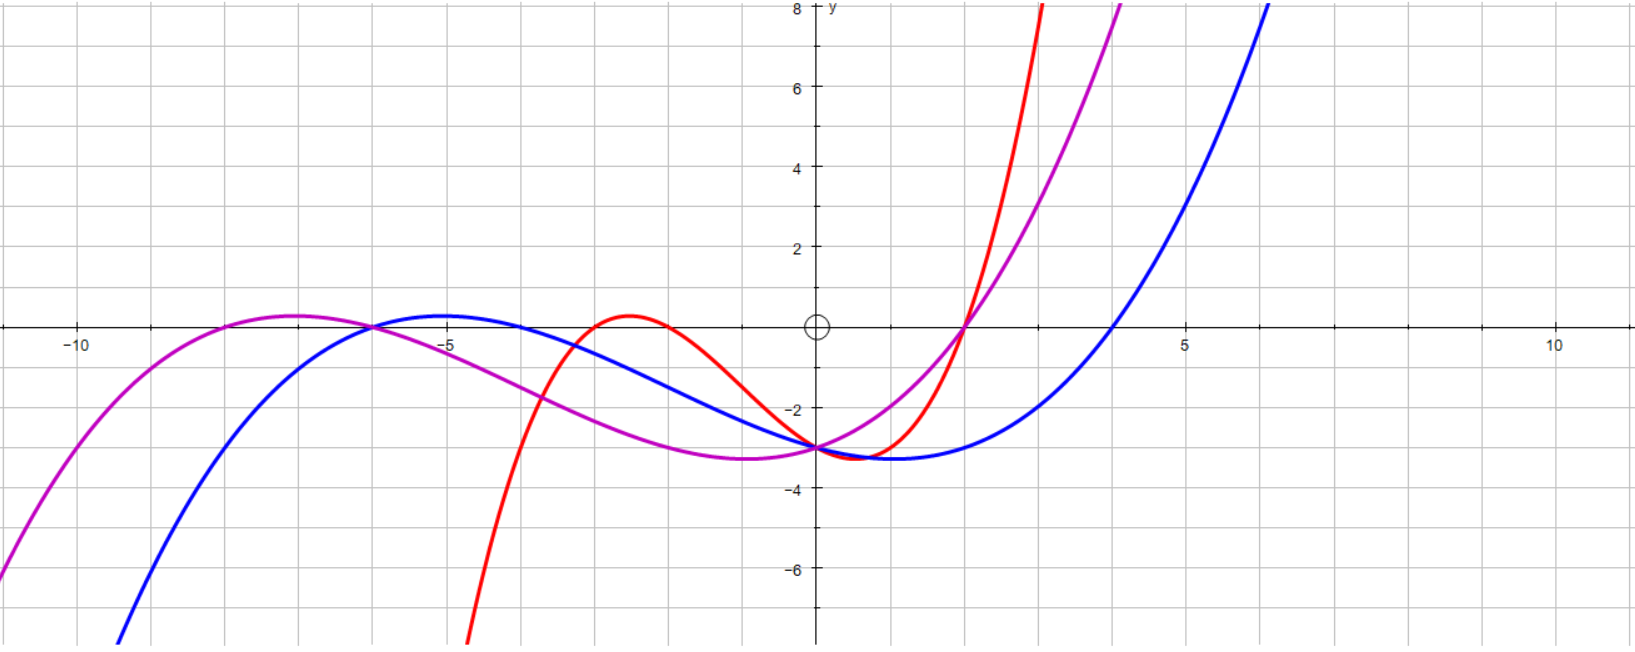
\includegraphics[width=\textwidth]{rootsofpolynomials}}
\end{figure}

\noindent
The roots of the \textcolor{red}{red} equation are $\alpha$, $\beta$ and $\gamma$; \newline
The roots of the \textcolor{blue}{blue} equation are $2\alpha$, $2\beta$ and $2\gamma$; \newline
The roots of the \textcolor{purple}{purple} equation are $2\alpha-1$, $2\beta-1$ and $2\gamma-1$; \newline \par

The \textcolor{purple}{purple} curve can be obtained by a sequence of transformations of the orginal, \textcolor{red}{red} curve.
\begin{itemize}
\item[]
\vspace{-0.25cm}
\begin{itemize}
\item[1)] Stretch in the $x$-direction by scale factor 2 (\textcolor{red}{$x$} $\rightarrow$ \textcolor{blue}{$\frac{1}{2}x$})
\vspace{-0.15cm}
\item[2)] Translation by vector \scriptsize $\begin{bmatrix}-1\\0\end{bmatrix}$ \normalsize (\textcolor{blue}{$x$} $\rightarrow$ \textcolor{purple}{$x+1$})
\end{itemize}
\end{itemize}

Therefore the original equation, 
\begin{equation*}
y=k(x-\alpha)(x-\beta)(x-\gamma)
\end{equation*}
can therefore be replaced by the substitution $x\rightarrow\frac{x+1}{2}$, to give
\begin{equation*}
y=k\left(\frac{x+1}{2}-\alpha\right)\left(\frac{x+1}{2}-\beta\right)\left(\frac{x+1}{2}-\gamma\right)
\end{equation*}
\vspace{-0.4cm}


\subsection{The modulus function}
\begin{itemize}
\item A Level M Year 2 \hspace{1cm} \phantom{ AS / } Pages 50 -- 59
\end{itemize} \par
The modulus function, $|x|$ gives the magnitude of a number. Graphs of modulus functions give a sharp turn\footnote{Unless the function never strictly crosses the $x$-axis, for example $f(x)=cos(x)+1$} at the $x$-axis, whereas a polynomial for instance may cut the axis. 
\vspace{-0.25cm}
\begin{align*}
|a|=|b| \;&\Longleftrightarrow\; a^{2}=b^{2} \;\Longleftrightarrow\; a=\pm b  \\
|x-a|<b \;&\Longleftrightarrow\; a-b<x<a+b  \\
x^{2} \leq y^{2} \;&\Longleftrightarrow\; |x|\leq |y| 
\end{align*}


\subsection{Loci}
\label{loci}
\begin{itemize}
\item A Level M AS / Year 1 \hspace{1cm} \phantom{ } Pages 87 -- 112
\end{itemize} \par
A locus (pl. loci) is a set of points which satisfy certain conditions, (e.g. a set of points a distance $a$ from the point $(x,y)$ is a circle of radius $a$ centred on $(x,y)$).
\vspace{0.5cm}


\subsection{Parametric curves}
\begin{itemize}
\item A Level M Year 2 \hspace{1cm} \phantom{ AS / } Pages 253 -- 258
\end{itemize} \par
Parametric curves are where the two axes are defined in terms of some other variable, for example
\vspace{-0.2cm}
\begin{align*}
x&=\cos(\theta) \\
y&=\sin(\theta)
\end{align*}
For the Cartesian form, these must be substituted in to give $y$ in terms of $x$, or vice versa.
\vspace{0.5cm}


\subsection{Polar coordinates}
\begin{itemize}
\item A Level M Year 2 \hspace{1cm} \phantom{ AS / } Pages 199 -- 209
\end{itemize}
Polar coordinates are defined in terms of the distance of the point from the origin (radius) and the anti-clockwise angle from the positive $x$-axis.
\begin{equation*}
\begin{Bmatrix} r, \mathrm{radius} \\ \theta, \mathrm{angular\; coordinate}\end{Bmatrix} \\
\end{equation*}
\begin{align*}
&\mathrm{Cartesian:} & &15=x^{2}+y^{2} \\
&\mathrm{Parametric:}&  &\begin{Bmatrix} x=2t-5 \\ y=3t \end{Bmatrix} \\
&\mathrm{Polar:}&  &r=a\left( 1+\frac{\theta}{\pi} \right)\text{ for } 0\leq\theta\leq2\pi\text{, }a>0
\end{align*}
\par
$r$ is constrained to $r\geq0$. The domain of $\theta$ is specified by context

\begin{figure}[H]
     \centering
         \scalebox{.8}{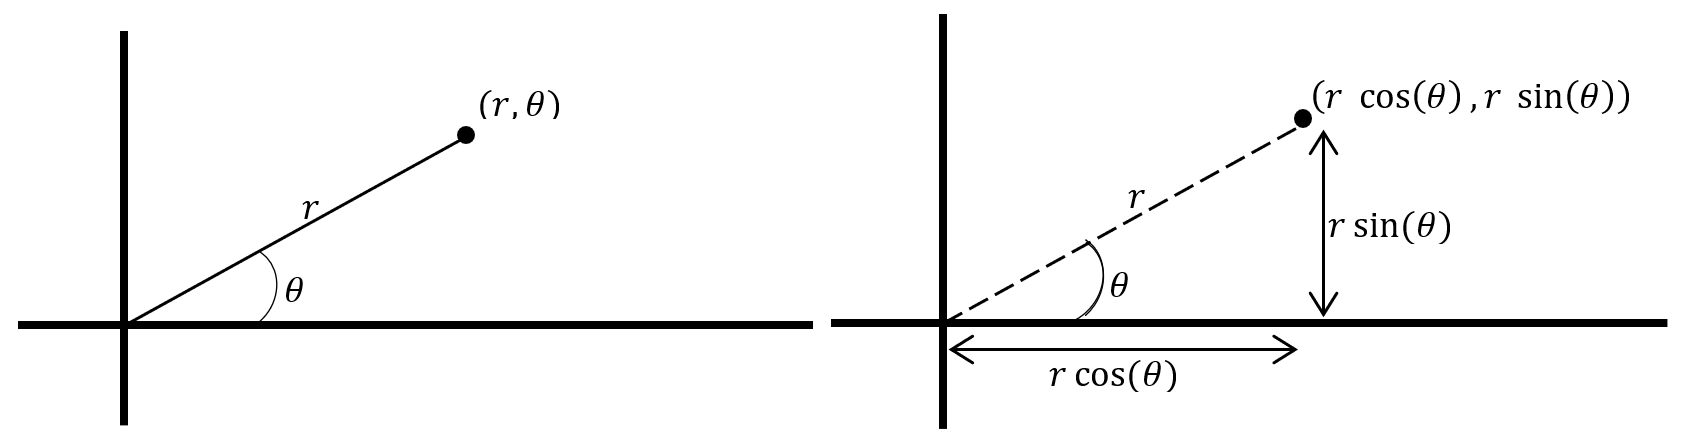
\includegraphics[width=\textwidth]{polarcoordinates}}
\end{figure}
To convert from polar $(r,\theta)$ to Cartesian form $(x,y)$,
\vspace{-0.2cm}
\begin{align*}
x&=r\cos(\theta) \\
y&=r\sin(\theta)
\end{align*}
To convert from Cartesian form $(x,y)$ to polar $(r,\theta)$
\begin{align*}
r&=\sqrt{x^{2} + y^{2}} \\
\theta&=\arctan\left(\frac{y}{x}\right)
\end{align*}
\vspace{0.5cm}


\end{document}